\section{ 永遠}

\parpic[r]{
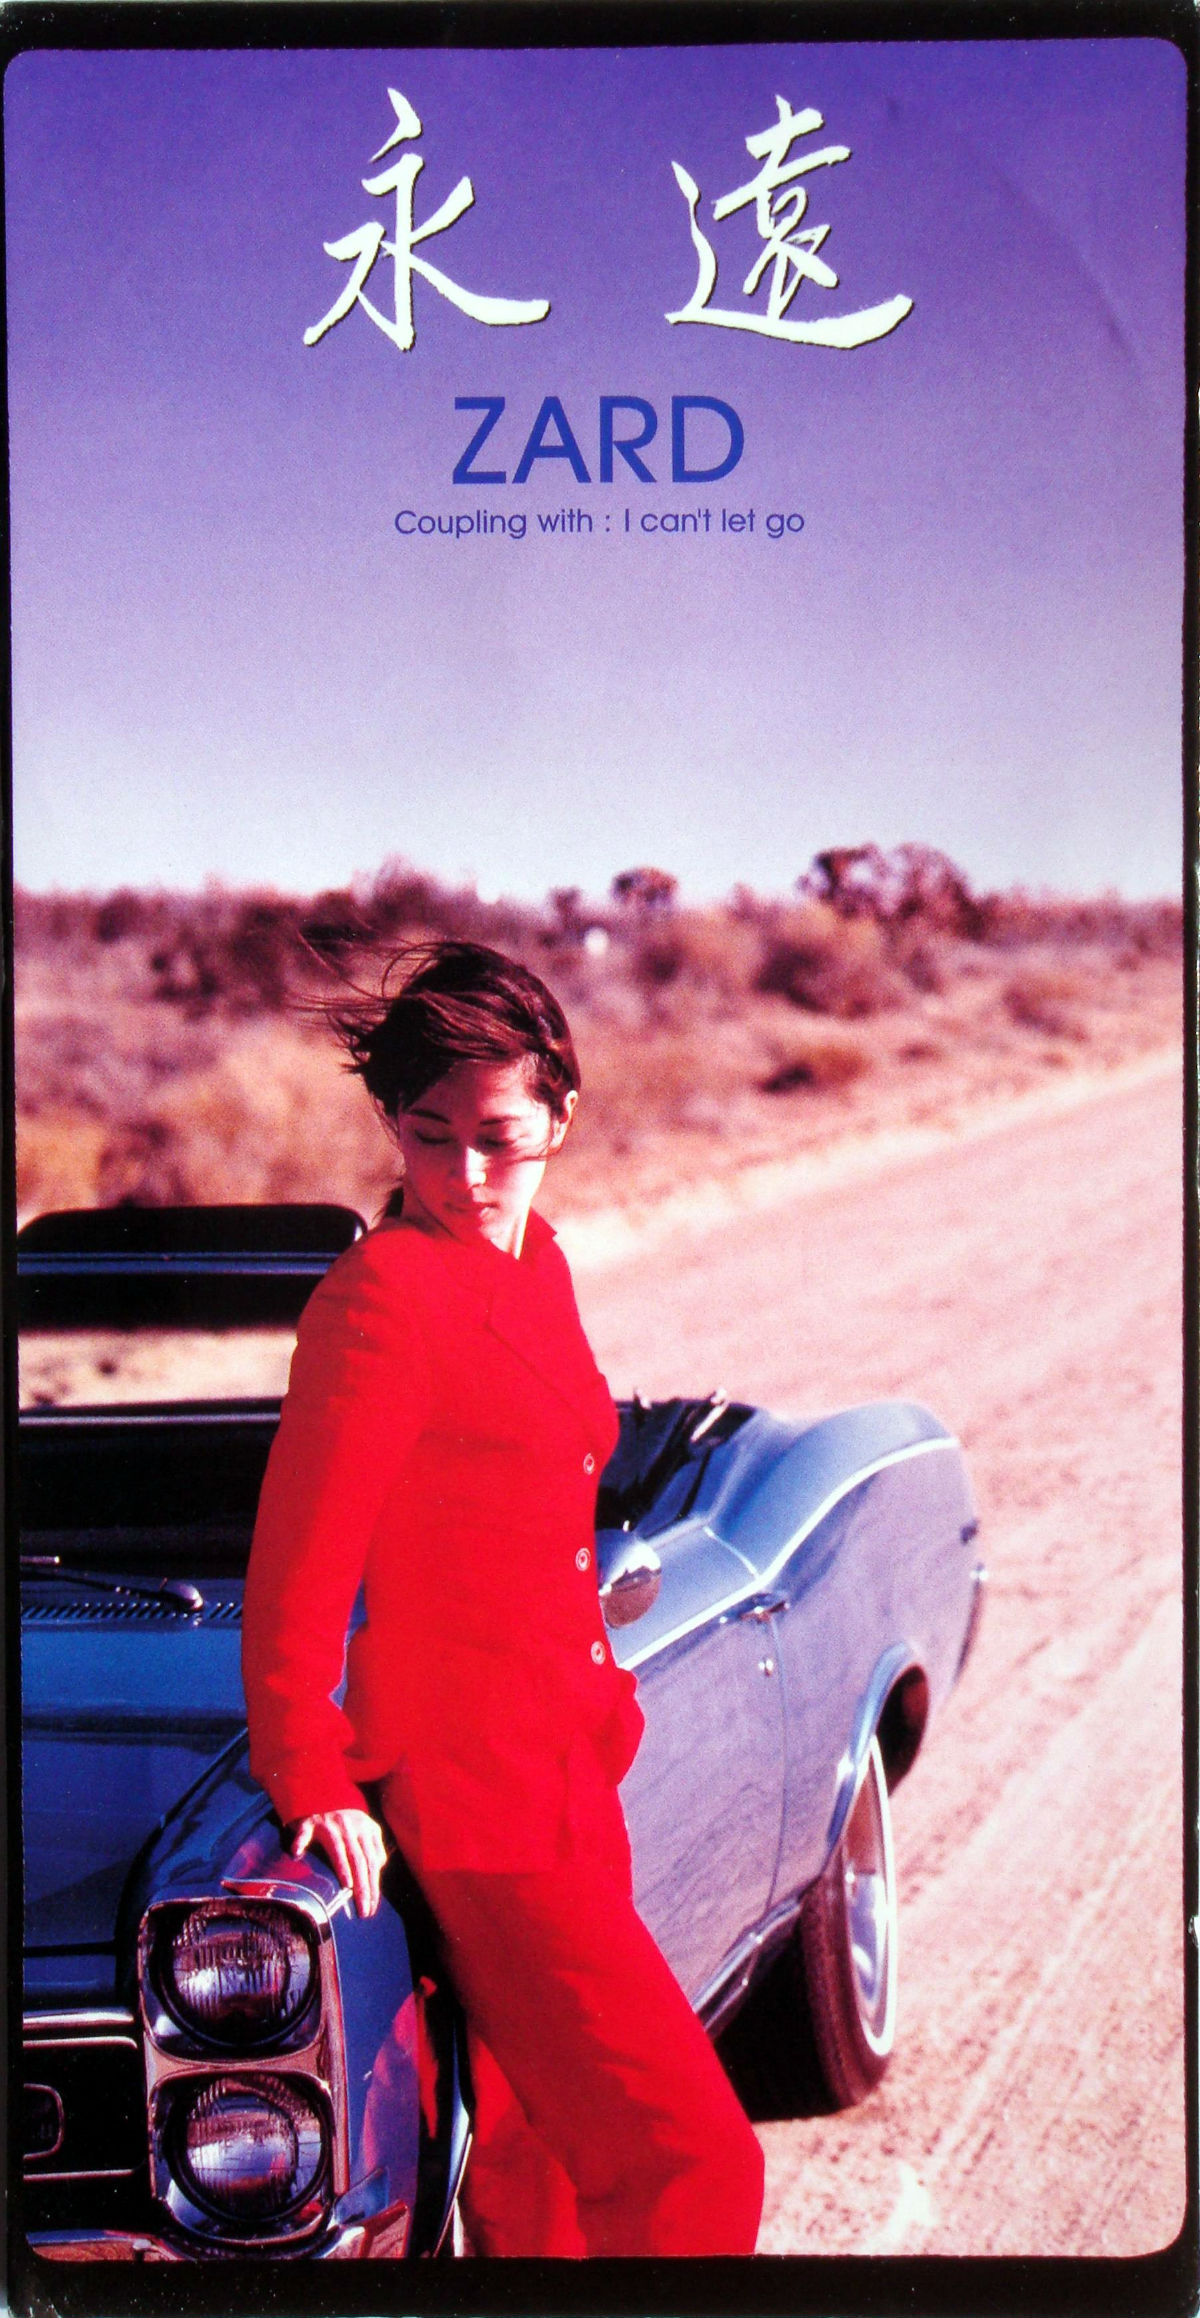
\includegraphics[width=0.3\textwidth]{S22.jpg}}

\large{

\ruby{朱}{あか}い\ruby{果実}{かじつ}を\ruby{見}{み}たら

\ruby{私}{わたし}のことを\ruby{思}{おも}い\ruby{出}{だ}してください

あなたの\ruby{決心}{けっしん}が\ruby{固}{かた}まったら…

きらきらと\ruby{ガラス}{Glass}の\ruby{粉}{かけら}になって

このまま \ruby{消}{き}えてしまいましょう 

\ruby{誰}{だれ}も\ruby{知}{し}らない\ruby{楽園}{くに}へ
\\

\ruby{今}{いま}の\ruby{二人}{ふたり}の\ruby{間}{あいだ}に 

\ruby{永遠}{えいえん}は\ruby{見}{み}えるのかな

すべてを \ruby{手}{て}に\ruby{入}{い}れることが \ruby{愛}{あい}ならば

もう\ruby{失}{うしな}うものなんて \ruby{何}{なに}も\ruby{怖}{こわ}くない
\\

\ruby{口}{くち}のきき\ruby{方}{かた}も\ruby{知}{し}らない 

\ruby{生意気}{なまいき}な\ruby{女性}{やつ}だと\ruby{思}{おも}った?

\ruby{偶然}{ぐうぜん} \ruby{街}{まち}で\ruby{見}{み}かけたけど 

\ruby{声}{こえ}をかけようかどうか\ruby{迷}{まよ}った

\ruby{守}{まも}るべきものは \ruby{何}{な}のか 

この\ruby{頃}{ころ} それが\ruby{分}{わ}からなくなる…
\\

「\ruby{君}{きみ}と\ruby{僕}{ぼく}との\ruby{間}{あいだ}に \ruby{永遠}{えいえん}は\ruby{見}{み}えるのかな」

どこまでも\ruby{続}{つづ}く\ruby{坂道}{さかみち}

あの\ruby{日}{ひ}から\ruby{淋}{さび}しかった 

\ruby{想像}{そうぞう}\ruby{以上}{いじょう}に… 

Just Fallin' of the Rain
\\

\ruby{君}{きみ}と\ruby{僕}{ぼく}との\ruby{間}{あいだ}に \ruby{永遠}{えいえん}は\ruby{見}{み}えるのかな

この\ruby{門}{もん}をくぐり\ruby{抜}{ぬ}けると

\ruby{安}{やす}らかなその\ruby{腕}{うで}にたどりつける

また\ruby{夢}{ゆめ}を\ruby{見}{み}る\ruby{日}{ひ}まで

}